\scanpage{89}\mspage{88}

Nous imposerons \unsure{du moins|de même} cette condition pour les ateliers \uline{saturés} (cf plus bas). Mais on notera que cette condition n\deleted{\unsure{'est}}e sera pas vérifiée dans \unsure{les|le} cas d'ateliers \deleted{\unsure{semi}} simpliciaux \inserted{\unsure{stricts|strict}}, par exemple
\figure{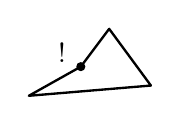
\begin{tikzpicture}[x=1cm,y=1cm,line join=round]
\draw[line width=.85pt] (0,0) -- (.66,.37) -- (1.02,.85) -- (1.55,.13) -- cycle;
\fill (.66,.37) circle[radius=1.65pt];
\node at (.42,.54) {$!$};
\end{tikzpicture}}
est un contre-exemple.

(Atelier simplicial : tout $X\in M$ est un ``simplexe combinatoire'', ou encore : \inserted{$\forall X\in M$,} \deleted{\unsure{toute}} partie \deleted{majorée} \inserted{non vide} de $\deleted{\unsure{M}}{\widetilde X}$ \inserted{(pour $\leq$)} \unsure{a} un sup, \inserted{\unsure{tout} élément non minimal a au moins \unsure{deux} prédécesseurs, $\unsure{\#|*}$} \deleted{\unsure{les}} et $\widetilde X$ \deleted{\unsure{sont}} \unsure{fini|finis}, \deleted{Attention \unsure{;|:} se \unsure{faut-il|peut-il} que tout \unsure{élém.} non minimal a au \unsure{moins} \unsure{deux} préd.} \deleted{toute partie finie \inserted{\unsure{non vide} majorée} de $M$ a un sup, et les $\widetilde X$ sont finis.]} pas que toute partie finie \unsure{majorée} de $M$ ait un sup, \unsure{(}ex :
\figure{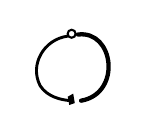
\begin{tikzpicture}[x=1cm,y=1cm,line cap=round]
\draw[line width=1.05pt] (.39,.86) .. controls (.09,.82) and (-.10,.50) .. (.04,.23) .. controls (.13,.09) and (.30,.05) .. (.43,.04);
\draw[line width=1.55pt] (.52,.88) .. controls (.98,.94) and (1.08,.13) .. (.56,.04);
\draw[fill=white,line width=.75pt] (.44,.89) circle[radius=1.45pt];
\fill (.41,-.015) -- (.48,.01) -- (.46,.13) -- (.39,.09) -- cycle;
\end{tikzpicture}}
)
\margin{Atelier simplicial strict : simplicial et $X\unsure{\mathrel{\mathord{\rlap{$>$}<}}|,|\mathrel{\lesseqgtr}}Y$ \unsure{compatible|compatibles} $\Longrightarrow X\cap Y$ \inserted{\unsure{ens}} $\in M$ i.e. : Si $\{X,Y\}$ \deleted{\unsure{vide}} \inserted{\unsure{minorée|minoré}}, $\unsure{\inf|\mathrm{Inf}}(X\unsure{.|,}Y)$ existe dans $M$}% slanted

Pour le moment, je voudrais

1$^\circ$) Expliciter les axiomes dans le cas d'un atelier ensembliste

2$^\circ$) Voir leur stabilité ou non stabilité par passage à un sous-atelier

3$^\circ$) Étudier l'opération de \uline{saturation} d'un atelier (en me restreignant au besoin au cas d'un atelier ``modéré'').

Nous avons vu (p. \unsure{55-53|55-57|56-53|55-55}) qu'un atelier ensembliste est défini par un ens $L$ et une partie \deleted{$\unsure{\mathcal F\subset|\mathcal F\in}$}
\[
\mathcal F\subset\mathrm{Fig}(L)
\]
satisfaisant les conditions $\unsure{\mathrm{At}\,\mathrm{ens}^{\alpha}|\mathrm{At}\,\mathrm{ens}^{a}}$ 1, 2, 3.

$\unsure{\hookrightarrow|G|\subset}$ On a déjà vu qu'on a alors automatiquement At 1 à At 8. Il faut examiner les autres axiomes. Pour les exemples et contre exemples on pensera surtout au cas $L$ fini, et où on \inserted{peut se reporter au point de}
